\chapter{Design und Implementierung der Klassifizierungspipeline}\label{ch:klassifizierungsalgorithmus-(design-und-implementierung)}

Dieses Kapitel beschreibt die Pipeline zur Klassifikation \ac{DSGVO}-kritischer Aktivitäten in \ac{BPMN}-Prozessen. Ausgehend von der in Kapitel \ref{sec:aufgabenstellung} formulierten Aufgabenstellung wird der gesamte Weg von der Eingabe eines \emph{BPMN-XML} über die Vorverarbeitung, das Prompt Engineering bis hin zur strukturierten, schema-konformen Ausgabe aufgezeigt. Außerdem wird ein HTTP-basiertes API-Design vorgestellt, das die Einbindung in weitere Werkzeuge und das Evaluationsframework ermöglicht. Der Prozessfluss der Klassifizierungspipeline ist in Abbildung \ref{fig:architecture-diagram} dargestellt und wird in diesem Kapitel im Detail erläutert.

\begin{figure}[h]
    \centering
    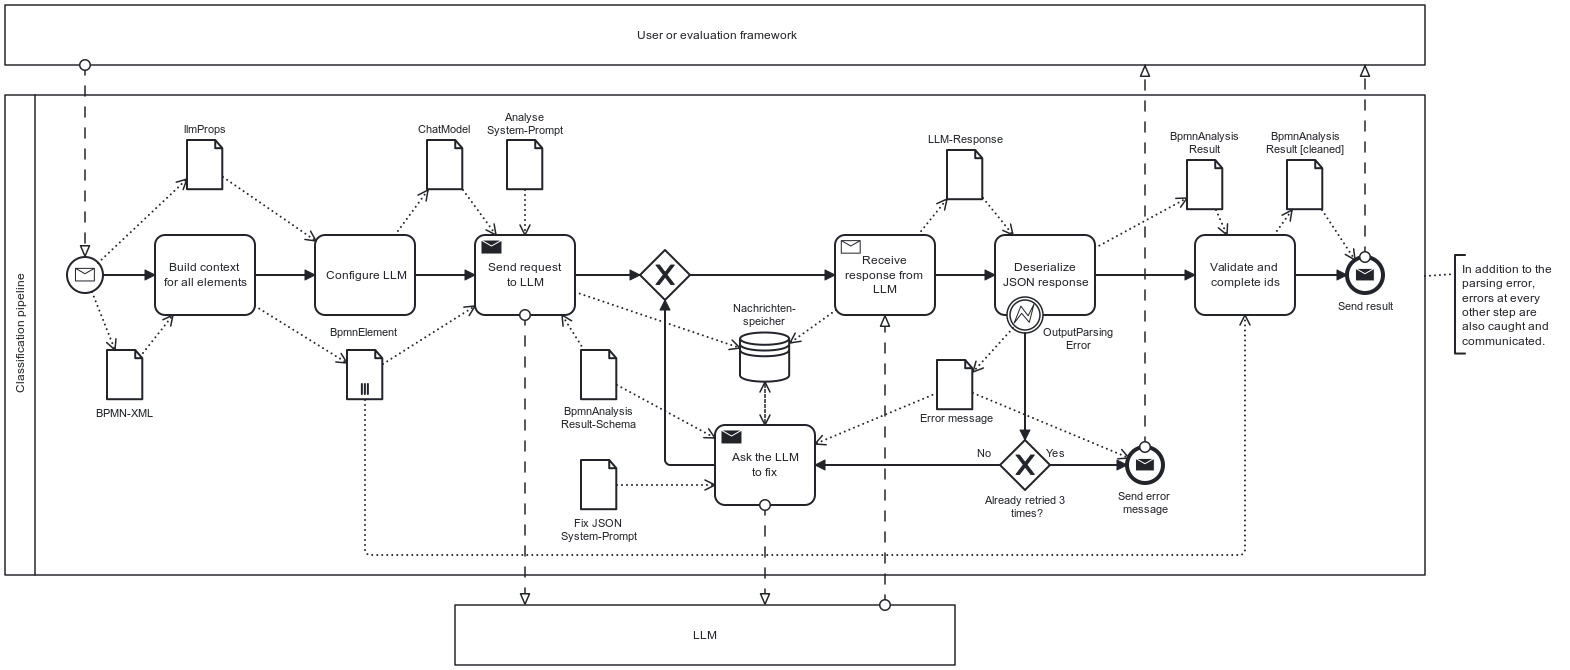
\includegraphics[width=\textwidth]{images/classification/classification-pipeline-diagram-en}
    \caption{\ac{BPMN}-Diagramm der Klassifizierungspipeline.}
    \label{fig:architecture-diagram}
\end{figure}

Die Klassifizierungspipeline soll eine binäre Entscheidung auf Ebene einzelner\linebreak\ac{BPMN}-Aktivitäten treffen: Für jede Aktivität eines Eingabemodells wird bestimmt, ob sie \emph{kritisch} im Sinne der \ac{DSGVO} ist. Die Pipeline ist so konzipiert, dass sie mit Modellen aus gängigen Modellierungswerkzeugen kompatibel ist. Dadurch kann sie in bestehende Modellierungswerkzeuge wie Camunda Modeler \cite{camunda} integriert werden, um einen praktischen Einsatz in realen Prozessmodellierungs-Workflows zu ermöglichen.

\section{BPMN Preprocessing}\label{sec:bpmn-preprocessing}

Ziel der Vorverarbeitung (Preprocessing) ist es, für jedes Flow-Element einen \emph{strukturierten Kontext} zu erzeugen. Dieser Kontext umfasst die eigenen Attribute, wie \texttt{id}, \texttt{name} und \texttt{documentation}, sowie die Beziehungen zu anderen Elementen im \ac{BPMN}-Diagramm. Dazu gehören vorangehende und nachfolgende Flow-Elemente, Datenobjekte, assoziierte Elemente, sowie Informationen über den Pool und die Lane, in denen sich das Element befindet. Das Parsen des \ac{BPMN}-XML erfolgt mit der \emph{Camunda BPMN Model API}, die das XML in ein Objektmodell überführt \cite{camunda-bpmn-model-api, camunda-bpmn-model-read}. Auf dieser Basis werden die relevanten Informationen extrahiert und in der Datenklasse \texttt{BpmnElement} strukturiert abgelegt. Die Datenklasse ist in Listing \ref{lst:bpmn-element-class} zu sehen. Dadurch entsteht für jedes Flow-Element ein umfassender Kontext, der später im Prompt genutzt wird, um dem \ac{LLM} alle notwendigen Informationen strukturiert bereitzustellen. Außerdem werden durch das Format Tokens eingespart, da irrelevante Informationen, wie die Positionen der Elemente im XML, weggelassen werden. In Abbildung \ref{fig:architecture-diagram} ist dieser Schritt über die Aktivität \enquote{Kontext aller Elemente aufbauen} dargestellt.

\begin{lstlisting}[language=Kotlin,caption={Interne \ac{BPMN}-Repräsentation je Flow-Element.},label={lst:bpmn-element-class}]
data class BpmnElement(
    val type: String,
    val id: String,
    val name: String? = null,
    val documentation: String? = null,
    val poolName: String? = null,
    val laneName: String? = null,
    val outgoingFlowElementIds: List<String> = emptyList(),
    val incomingFlowElementIds: List<String> = emptyList(),
    val outgoingMessageFlowsToElementIds: List<String> = emptyList(),
    val incomingMessageFlowsFromElementIds: List<String> = emptyList(),
    val incomingDataFromElementIds: List<String> = emptyList(),
    val outgoingDataToElementIds: List<String> = emptyList(),
    val associatedElementIds: List<String> = emptyList()
)
\end{lstlisting}
\section{Prompt Engineering}\label{sec:prompt-engineering}

Eine robuste Klassifikation hängt maßgeblich von sorgfältig gestalteten Prompts ab. Ziel ist es, das \ac{LLM} mit klaren Anweisungen, einem konsistenten Bewertungsschema und präzisen Formatvorgaben so zu steuern, dass es die Klassifizierung zuverlässig löst und strukturierte Ausgaben liefert. Im Folgenden werden zunächst die deklarative Orchestrierung der Kommunikation mit dem \ac{LLM} mithilfe von LangChain4j und anschließend die Prompt-Konzeption beschrieben.

\subsection*{LangChain4j: deklarative Orchestrierung}
Zur Reduktion von Boilerplate und für konsistente Prompts wird \emph{LangChain4j} \cite{langchain4j} benutzt. Mit den \emph{AI Services} werden Interaktionen mit dem \ac{LLM} als Java/Kotlin-Interface \emph{deklarativ} beschrieben. Zur Laufzeit erzeugt LangChain4j einen Proxy, der den System-Prompt injiziert, den User-Prompt aus den Methodenparametern generiert und die \ac{LLM}-Antwort in den passenden Rückgabetyp deserialisiert \cite{langchain4j-ai-services}. Beim erstellen des AI Service werden ein \texttt{ChatModel}, die Systemnachricht und die Interface-Methoden konfiguriert. Ein \texttt{ChatModel} ist die spezifische Implementierung der Chat-Completion-Schnittstelle eines \ac{LLM} von Langchain4j \cite{langchain4j-chat-model}. Die Methodenparameter der Interface-Methoden repräsentieren die Nutzereingabe. Der Rückgabetyp der Methoden definiert die erwartete Antwortstruktur des \ac{LLM}. Optional kann jeder Interface-Methode noch ein eigener User-Prompt zugewiesen werden, der bei Laufzeit mit den übergebenen Parametern gefüllt wird \cite{langchain4j-ai-services}.

Die Kommunikation mit dem \ac{LLM} erfolgt damit über einfache Funktionsaufrufe, während LangChain4j Prompt-Erzeugung, Parameterbindung sowie die Deserialisierung der Antwort übernimmt \cite{langchain4j-ai-services}. So kann im Code ohne zusätzlichen Aufwand direkt mit typisierten Objekten gearbeitet werden.

Für die Klassifikation \emph{\ac{DSGVO}-kritisch vs.\ unkritisch} wird ein \textbf{Zero-Shot}-Ansatz verwendet. Das \ac{LLM} erhält im System-Prompt eine präzise Instruktion mit Kriterien und illustrativen Beispielfällen, was als kritisch gilt. Es sind jedoch keine Beispiele mit konkreten Ein- und Ausgabe-paaren pro Prozess enthalten. Zero-Shot reduziert den Pflegeaufwand und nutzt die In-Context-Fähigkeiten moderner Modelle, nur über Instruktionen zu generalisieren \cite{brown2020fewshot,liu2023prompting}. Wie genau die Prompts aufgebaut sind, wird im Folgenden beschrieben.

\subsection*{System-Prompt}

Der System-Prompt definiert das Verhalten des \ac{LLM}, zusätzlichen Kontext und das gewünschte Ausgabeformat. Der vollständige System-Prompt befindet sich im Anhang, siehe \ref{lst:system-prompt}. Im Kern legt der genutzte System-Prompt Folgendes fest:

\begin{enumerate}
    \item \textbf{Rolle und Auftrag des Modells.} Das Modell agiert als Experte für das Analysieren von \ac{BPMN}-Modellen auf \ac{DSGVO}-konformität und prüft sämtliche Aktivitäten eines Prozesses auf Datenschutzrelevanz. Jede Aktivität wird berücksichtigt und die Entscheidung erfolgt auf Basis sämtlicher verfügbarer Kontextinformationen wie Name, Beschreibung, Annotationen sowie Daten- und Nachrichtenassoziationen.
    \item \textbf{Rechtliche Definitionen nach \ac{DSGVO}.} Der System-Prompt erläutert die Begriffe \enquote{personenbezogene Daten} und \enquote{Verarbeitung} gemäß Art.\,4 \ac{DSGVO}. Beispiele für personenbezogene Daten umfassen Identifikatoren, Kontakt- und Zahlungsdaten, Beschäftigungsdaten, Gesundheitsdaten, biometrische Merkmale, Standortinformationen und Online-Kennungen. Verarbeitung umfasst Erheben, Speichern, Abrufen, Verwenden, Übermitteln, Ausrichten, Kombinieren, Einschränken, Löschen und Vernichten.
    \item \textbf{Indikatoren für Kritikalität.} Der System-Prompt enthält typische Auslöser für Datenschutzrelevanz wie Datenerfassung und Dateneingabe, Anlage und Aktualisierung von Datensätzen, Übermittlung oder Offenlegung an andere Systeme oder Dritte, Zahlungen und Finanztransaktionen und noch mehr. Diese Indikatoren sind mit Beispielen angereichert und dienen als \emph{Entscheidungshelfer} für das Modell.
    \item \textbf{Abgrenzung durch Negativbeispiele.} Der System-Prompt grenzt unkritische Fälle klar ab. Rein administrative oder logistische Schritte ohne Personenbezug werden nicht als kritisch gewertet. Ebenso gilt dies für Fälle in denen anonymisierte Daten verwendet werden und keine Identifikation einer Person mehr möglich ist.
    \item \textbf{Erwartetes Ausgabeformat.} Die Antwort erfolgt als strukturierte JSON-\hspace{0pt}Ausgabe mit einer Liste relevanter Aktivitäten. Für jede Aktivität wird die \texttt{id} und eine Begründung in natürlicher Sprache ausgegeben. Es werden ausschließlich Aktivitäten zurückgegeben, die nach den Kriterien als datenschutzrelevant eingestuft wurden.
\end{enumerate}

Die Kombination dieser Elemente im System-Prompt stellt sicher, dass das \ac{LLM} die Aufgabe versteht, die relevanten Kriterien kennt und die Ausgabe in einem maschinenlesbaren Format liefert. So entsteht die Basis für eine zuverlässige Klassifikation. Zu einer Anfrage an ein \ac{LLM} gehört außerdem stets ein User-Prompt, der die eigentliche Nutzereingabe enthält. Dessen Aufbau wird im nächsten Abschnitt beschrieben.

\subsection*{User-Prompt}

Der User-Prompt übergibt dem \ac{LLM} die konkreten Eingabedaten einer Anfrage. Während der System-Prompt Regeln, Ziele und Ausgabevorgaben festlegt, liefert der User-Prompt die Fall- bzw.\ Kontextinformationen, auf die diese Regeln angewendet werden.

Der User-Prompt wird mithilfe der Daten aus der Vorverarbeitung aus Abschnitt \ref{sec:bpmn-preprocessing} erzeugt und enthält eine Liste von \texttt{BpmnElement}-Objekten, siehe Listing~\ref{lst:bpmn-element-class}. Die Interaktion mit dem \ac{LLM} erfolgt deklarativ über \emph{LangChain4j}. Dafür wird die Liste der \texttt{BpmnElement}-Objekte als Methodenparameter mit der Annotation \texttt{@UserMessage} an die Interface-Methode übergeben und dort automatisch in den User-Prompt eingebettet.

Zur Laufzeit serialisiert \emph{LangChain4j} die \texttt{BpmnElement}-Liste zu einem JSON-Array und stellt sie als User-Prompt bereit. Der zuvor konfigurierte System-Prompt wird bei einer Anfrage an das \ac{LLM} automatisch dem User-Prompt vorangestellt. Auf diese Weise wendet das \ac{LLM} die im System-Prompt definierten Kriterien auf die im User-Prompt gelieferten Informationen zum \ac{BPMN}-Prozessmodell an. Dadurch wird jede Aktivität des Prozesses genau so wie im System-Prompt beschrieben klassifiziert. In Abbildung \ref{fig:architecture-diagram} findet dieser Schritt in der Aktivität \enquote{Anfrage an das LLM schicken} statt.

Zusammenfassend setzt der System-Prompt typischerweise das Regelwerk, und der User-Prompt liefert die konkreten Eingabedaten. Besonders in mehrstufigen Dialogen mit dem \ac{LLM} spielt dieses Muster eine größere Rolle, da der System-Prompt konstant bleibt, während der User-Prompt je nach Anfrage variiert. Im vorliegenden Szenario, wo immer nur genau eine Anfrage pro Prozessmodell gestellt wird fällt der Unterschied weniger ins Gewicht, als würden sämtliche Vorgaben direkt im User-Prompt stehen. Die Trennung erhöht dennoch die Nachvollziehbarkeit, sorgt für klare Rollen und erleichtert die Wiederverwendung.

Im folgenden Abschnitt wird beschrieben, wie auf dieser Basis strukturierte Ausgaben erzeugt werden, damit im Code direkt mit typisierten Objekten weitergearbeitet werden kann.

\subsection*{Strukturierte Ausgaben mit LangChain4j}

Wie in Listing \ref{lst:ai-service-interface} zusehen, wird im Fall der Klassifikation ein \texttt{BpmnAnalysisResult} als Antwort erwartet, also eine Liste von Elementen mit Paaren aus \texttt{id}, \texttt{reason} und \texttt{isRelevant}. Siehe \ref{lst:bpmn-analysis-result} für die vollständige Definition der Datenklasse. Langchain4j inferiert auf Basis des Rückgabetyps der Interface-Methode ein JSON-Schema und fügt dieses automatisch dem User-Prompt zusammen mit der Aufforderung hinzu, die Antwort in diesem JSON-Format zu liefern \cite{langchain4j-ai-services}. Durch die explizite Angabe des gewünschten JSON-Formats im Prompt wird die Format-Treue der Antwort erhöht \cite{liu2023prompting}, also die Wahrscheinlichkeit, dass die Antwort tatsächlich dem gewünschten Schema entspricht.

Einige \acp{LLM} unterstützen darüber hinaus die Möglichkeit, das Antwortformat API-seitig zu erzwingen. Das ist beispielsweise bei Mistral und OpenAI der Fall \cite{mistralai_structured_output, openai_structured_output}.
Falls das \ac{LLM} die \texttt{response\_format} Funktionalität unterstützt setzt LangChain4j dies zusätzlich auf das gewünschte Schema und erzwingt so das Ziel-JSON API-seitig \cite{langchain4j-ai-services}. Fehlt diese Fähigkeit, greift ausschließlich die Prompt-basierte Schemaanweisung.

Das vom \ac{LLM} gelieferte JSON deserialisiert \emph{LangChain4j} anschließend automatisch zu einem \texttt{BpmnAnalysisResult}. So kann im Code direkt mit einem typsicheren Objekt weitergearbeitet werden. In Abbildung \ref{fig:architecture-diagram} ist dieser Prozess über die Aktivitäten \enquote{Antwort von LLM erhalten} und \enquote{Antwort JSON deserialiseren} dargestellt.

\section{Validierung der Ausgabe}\label{sec:validierung-der-ausgabe}

Zusätzlich zu den in Kapitel \ref{sec:prompt-engineering} beschriebenen Maßnahmen zur Sicherstellung strukturierter Ausgaben wird die Antwort des \ac{LLM} durch LangChain4j validiert. Wenn das erwartete Schema vom \ac{LLM} nicht eingehalten wird, wirft Langchain4j eine \texttt{OutputParsingException}.

\textcolor{orange}{// TODO Eventuell noch Retry Mechanismus wenn am Ende noch Zeit ist mit Nachrichtenverlauf und Parsing Fehlermeldung. Das muss aber auch erst einmal implementiert werden. Aktuell gibt es nur den Parsing Error.}

Ein weiterer Mechanismus zur Validierung der Ausgabe ist die Überprüfung der ausgegebenen \texttt{ids}. Da das \ac{LLM} theoretisch jede beliebige \texttt{id} ausgeben könnte, werden die ausgegebenen \texttt{ids} mit den tatsächlichen \texttt{ids} der Aktivitäten aus dem Prozess abgeglichen. Falls eine ausgegebene Aktivität nicht im Prozess existiert, wird diese aus der Antwort der Klassifizierung entfernt. Dadurch wird sichergestellt, dass nur gültige \texttt{ids} in der finalen Ausgabe enthalten sind.
\section{API-Design}\label{sec:api}

Dieses Kapitel beschreibt das API-Design der Klassifizierungspipeline, die zur Erkennung \ac{DSGVO}-kritischer Elemente in \ac{BPMN}-Modellen dient. Das Ziel ist es eine standardisierte Schnittstelle zu definieren, um

\begin{enumerate}
    \item die Einbindung in bestehende Werkzeuge und das Evaluationsframework (siehe Kapitel \ref{ch:evaluationsframework}) zu vereinfachen,
    \item die Austauschbarkeit unterschiedlicher Klassifizierungsalgorithmen - insbesondere im Evaluationsframework - zu ermöglichen, um verschiedene Ansätze vergleichen zu können, und
    \item Erweiterbarkeit zu fördern, sodass zukünftige Arbeiten die Schnittstelle wiederverwenden können, um ihre eigenen Klassifizierungsalgorithmen zu integrieren.
\end{enumerate}

\subsection*{HTTP-Endpunkt}

Die Klassifizierungspipeline ist über einen HTTP-Endpunkt nutzbar. Der \texttt{POST}-Endpunkt akzeptiert \texttt{multipart/form-data} mit den folgenden Teilen:

\begin{description}
    \item[\texttt{bpmnFile} (Pflicht)] Eine BPMN-2.0-XML-Datei (\texttt{.bpmn} oder \texttt{text/xml}), die den zu analysierenden Prozess beinhaltet.
    \item[\texttt{llmProps} (Optional)] Ein JSON-Objekt zur Überschreibung von \ac{LLM}-Eigenschaften zur Laufzeit. Siehe Listing \ref{lst:api-request-schema} für das JSON-Schema. Wird nichts angegeben, nutzt die Pipeline Standardwerte.
\end{description}

Die \texttt{llmProps} erlauben es, verschiedene \acp{LLM} und deren Konfigurationen flexibel zu für die Klassifizierung zu nutzen, ohne die Anwendung neu starten zu müssen. Dies ist besonders nützlich im Evaluationsframework, um verschiedene Modelle zu vergleichen.

\begin{lstlisting}[language=json,caption={JSON-Schema der \texttt{llmProps}.},label={lst:api-request-schema}]
{
  "$schema": "https://json-schema.org/draft/2020-12/schema",
  "title": "LlmProps",
  "type": "object",
  "properties": {
    "baseUrl": {"type": "string"},
    "modelName": { "type": "string" },
    "apiKey": { "type": "string" },
    "timeoutSeconds": { "type": "number" },
    "seed": { "type": "number" }
  },
  "required": []
}
\end{lstlisting}

Die Antwort des Endpunkts wird als \texttt{application/json} geliefert und enthält eine Liste der als \ac{DSGVO}-kritisch klassifizierten Elemente, einschließlich einer optionalen Begründung für jede Klassifikation und einem optionalen Namen des Elements für bessere Lesbarkeit. Das JSON-Schema der API-Antwort ist in Listing \ref{lst:api-response-schema} dargestellt.

\begin{lstlisting}[language=json,caption={JSON-Schema der API-Antwort.},label={lst:api-response-schema}]
{
  "$schema": "https://json-schema.org/draft/2020-12/schema",
  "title": "BpmnAnalysisResult",
  "type": "object",
  "properties": {
    "criticalElements": {
      "type": "array",
      "items": {
        "type": "object",
        "properties": {
          "id": { "type": "string" },
          "name": { "type": "string" },
          "reason": { "type": "string" }
        },
        "required": ["id"]
      }
    }
  },
  "required": ["criticalElements"]
}
\end{lstlisting}

Ein Beispielaufruf des Klassifizierungsendpunkts mit \texttt{curl} könnte wie in Listing \ref{lst:api-curl-example} aussehen. Dabei wird eine BPMN-Datei hochgeladen und einige \ac{LLM}-Eigenschaften zur Laufzeit überschrieben, damit das Modell \texttt{mistral-small-latest} von Mistral AI verwendet wird.

\begin{lstlisting}[language=bash,caption={Beispielaufruf des Klassifizierungsendpunkts mit \texttt{curl}.},label={lst:api-curl-example}]
curl -X POST http://localhost:8080/gdpr/analysis/prompt-engineering \
    -F 'bpmnFile=@/path/to/process.bpmn' \
    -F 'llmProps={
        "baseUrl": "https://api.mistral.ai/v1/chat/completions",
        "modelName": "mistral-small-latest",
        "apiKey": "******"
    }'
\end{lstlisting}

\subsection*{Integration und Erweiterbarkeit}

Die gewählte API-Struktur mit einem standardisierten HTTP-Endpunkt und klar definierten JSON-Schemas ermöglicht eine einfache Integration in bestehende Werkzeuge und das Evaluationsframework (siehe Kapitel \ref{ch:evaluationsframework}). Durch die Möglichkeit, verschiedene \ac{LLM}-Eigenschaften zur Laufzeit zu überschreiben, können unterschiedliche Modelle mit einem Klassifizierungsalgorithmus flexibel getestet und verglichen werden, ohne die Anwendung neu starten zu müssen.

Zukünftige Arbeiten können die gleiche API nutzen, um ihre eigenen Klassifizierungsalgorithmen zu integrieren und so eine Vergleichbarkeit der Ergebnisse zu gewährleisten.
\section{Nutzung über Webapp}\label{sec:nutzung-uber-webapp}

Zur interaktiven Nutzung der Klassifizierung wurde eine \emph{Sandbox} in Form einer Webapp entwickelt. Sie verbindet einen vollwertigen \ac{BPMN}-Editor auf Basis von \texttt{BPMN.js} \cite{bpmn-js} mit der in Kapitel~\ref{sec:api-design} beschriebenen HTTP-Schnittstelle und macht die Analyse damit ganz einfach bedienbar. In der Sandbox können \ac{BPMN}-Modelle erstellt, verändert, exportiert und importiert sowie auf Datenschutzrelevanz analysiert werden. Als kritisch klassifizierte Aktivitäten werden nach der Analyse direkt im Editor farblich hervorgehoben, wie in Abbildung \ref{fig:sandbox-frontend-analyzed-model} zu sehen.

\begin{figure}
    \centering
    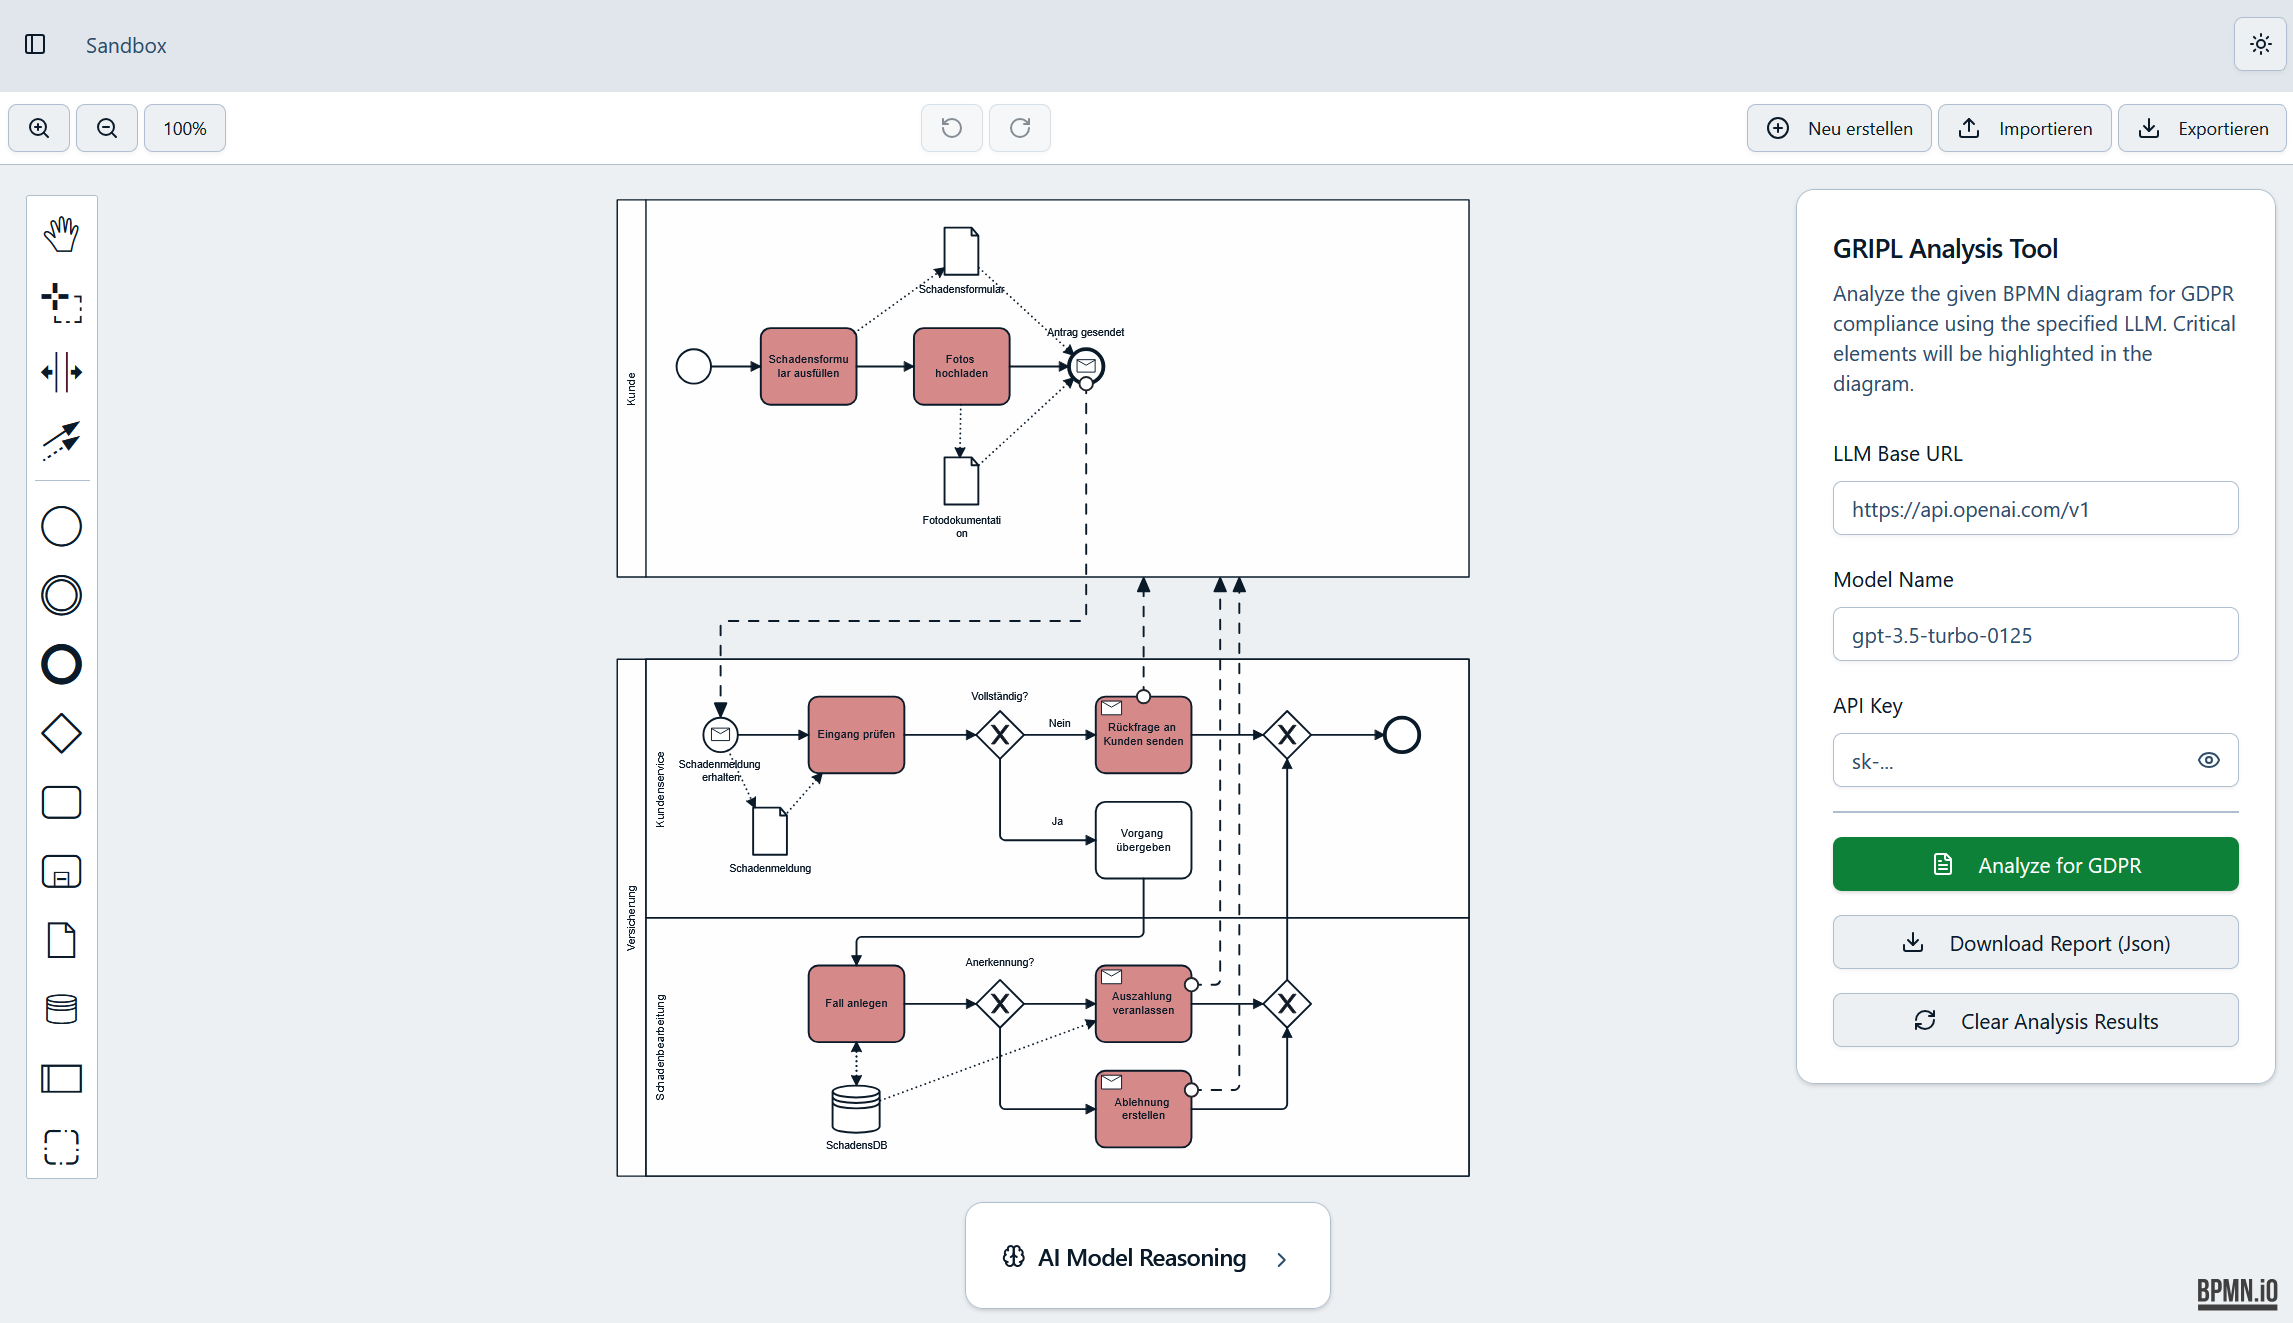
\includegraphics[width=\linewidth]{images/sandbox/sandbox-analyzed-model}
    \caption{Sandbox im Frontend mit hervorgehobenen kritischen Aktivitäten nach Analyse.}
    \label{fig:sandbox-frontend-analyzed-model}
\end{figure}

Außerdem können die vom \ac{LLM} generierten Begründungen zu jeder als kritisch erkannten Aktivität im Editor eingesehen werden. Diese Erläuterungen werden gesammelt in einer aufklappbaren Karte im unteren Bereich des Editors angezeigt, siehe Abbildung \ref{fig:sandbox-frontend-ai-reasoning}.

\begin{figure}
    \centering
    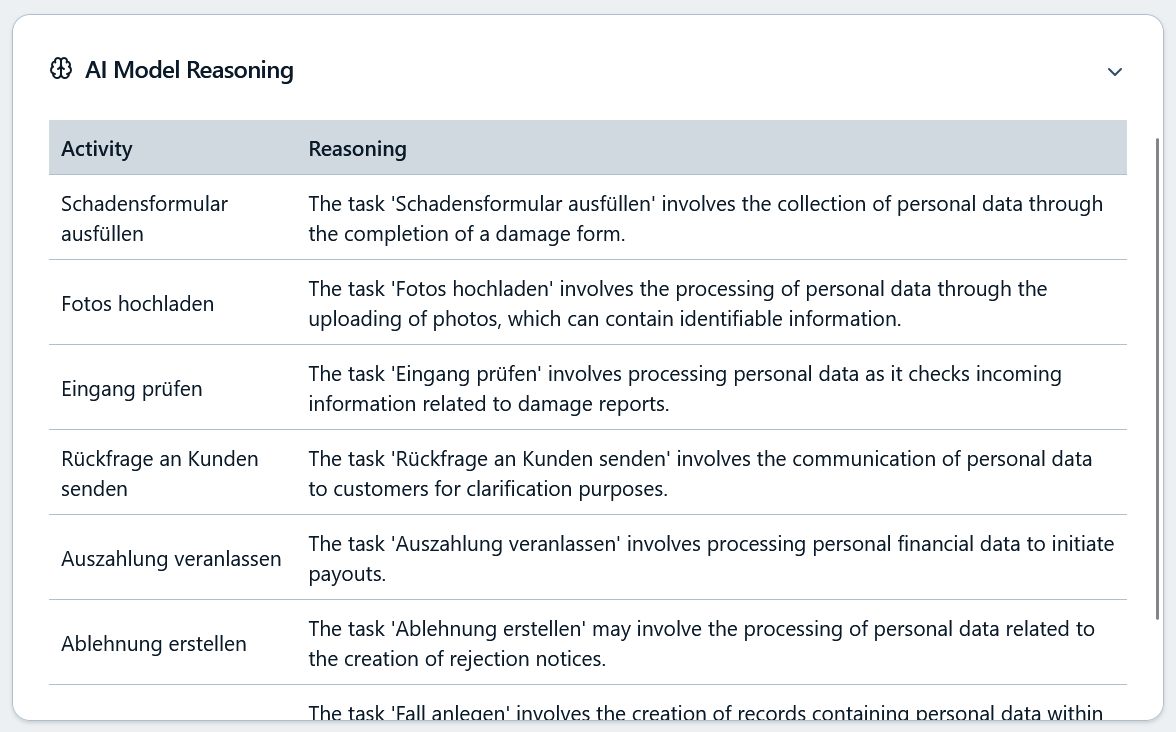
\includegraphics[width=\linewidth]{images/sandbox/sandbox-ai-reasoning}
    \caption{Begründung der Klassifikation durch das LLM in der Sandbox.}
    \label{fig:sandbox-frontend-ai-reasoning}
\end{figure}

Um verschiedene \acp{LLM} vergleichen zu können, verfügt die Sandbox auf der rechten Seite über ein Einstellungsmenü mit konfigurierbaren \ac{LLM}-Parametern (siehe Abbildung \ref{fig:sandbox-frontend-analyzed-model}). Diese Parameter sind identisch zu den in Kapitel \ref{sec:api-design} beschriebenen \texttt{llmProps} und werden beim Starten der Analyse in die API-Anfrage überführt.

